\documentclass{beamer}

\usepackage{lipsum}
\usepackage[orientation=landscape,size=a0,scale=1.2]{beamerposter}
\usepackage{amsmath,amsthm, amssymb}
\usepackage{setspace}
\setstretch{1}
%\boldmath

%\title[Beamer Poster]{Overleaf example of the beamerposter class}
%\author[welcome@overleaf.com]{Overleaf Team}
%\institute[Overleaf University]
%{The Overleaf institute, Learn faculty}
%\date{\today}

\graphicspath{{images/}}
\usepackage{hyperref}
\hypersetup{
	colorlinks=true,
	linkcolor=blue,
	filecolor=magenta,      
	urlcolor=cyan,
}
%\logo{\includegraphics[height=7.5cm]{example-image-a}}
\usetheme[]{default}

\setbeamertemplate{navigation symbols}{}
\definecolor{main}{HTML}{750f6d}
%\setbeamercolor*{palette primary}{bg=white}
\definecolor{background}{RGB}{250, 250, 250}
\definecolor{cuhk yellow}{RGB}{211, 163, 0}
%\definecolor{alert}{RGB}{}
\setbeamercolor{block title}{bg=main, fg=cuhk yellow}
\setbeamercolor{block body}{bg=main!1!background, fg=black}

\setbeamertemplate{caption}[numbered]
\setbeamercolor{alerted text}{fg=main}

\setbeamertemplate{bibliography item}[text]
\setbeamertemplate{bibliography entry title}{}
\setbeamertemplate{bibliography entry location}{}
\setbeamertemplate{bibliography entry note}{}
\setbeamerfont{bibliography item}{size=\scriptsize}
\setbeamerfont{bibliography entry author}{size=\scriptsize}
\setbeamerfont{bibliography entry title}{size=\scriptsize}
\setbeamerfont{bibliography entry location}{size=\scriptsize}
\setbeamerfont{bibliography entry note}{size=\scriptsize}
%\footlineinfo{123}
%\setbeamercolor{footline}{fg=main, bg=main}  % Disable the page number
\setbeamertemplate{headline}{
	\begin{beamercolorbox}[wd=\paperwidth]{headline}
		\begin{columns}
			\begin{column}{0.125\linewidth}
				\hspace{\fill}
				\centering
				\includegraphics[width=0.85\linewidth]{cuhk-emblem}
			\end{column}
			\begin{column}{0.75\linewidth}
				\vspace{5mm}
				
				\centering\bfseries
				{\fontsize{70}{84}\selectfont Optimal Sensor Fusion using $\mathcal{H}_\infty$ methods} \\ {\fontsize{60}{72}\selectfont Synthesizing Complementary Filters for Active Seismic Noise Isolation Systems in KAGRA}\\[5mm]
				\mdseries
				{\fontsize{60}{72}\selectfont Terrence T.L. Tsang on behalf of the KAGRA Collaboration} \\[5mm]
				{\fontsize{40}{48}\selectfont The Chinese University of Hong Kong. Email: \href{mailto:ttltsang@link.cuhk.edu.hk}{ttltsang@link.cuhk.edu.hk}}
			\end{column}
			\begin{column}{0.125\linewidth}
				\centering
				\includegraphics[width=0.85\linewidth]{KAGRA-logo}
				\hspace{\fill}
			\end{column}
		\end{columns}
	\end{beamercolorbox}
%\color{main!80!background}\rule{\paperwidth}{20pt}
}


\begin{document}
\begin{frame}[t]
%	\begin{abstract}
%		\lipsum[1]
%	\end{abstract}
	\begin{columns}[t]
		
		% Column 1
		\begin{column}{0.32\linewidth}
			
			\begin{block}{Introduction: Vibration Isolation Systems and Complementary Filters}
%				Seismic isolation for ground-based interferometric gravitation-wave detectors plays a crucial  role for suppressing the displacement level of the main optics so 1) the main optics are sufficiently stable to not cause lock-loss of the interferometer, and 2) displacement noise at detection band ($>10\,\text{Hz}$) does not compromise the sensitivity of the detector.
%				\begin{enumerate}
%					\item the main optics are sufficiently stable to not cause lock-loss of the interferometer, and 
%					\item displacement noise at detection band (> 10 Hz) does not compromise the sensitivity of the detector.
%				\end{enumerate}
				\medskip
				
				\begin{columns}[t, onlytextwidth]
					\begin{column}{0.47\textwidth}	
%						At higher frequencies, the displacement of the optics due to seismic noise is suppressed passively by suspending the optics with multiple-stage pendulum (suspension).
%						At lower frequencies, the residual motion of the optics is dominated by resonances excited by the ground motion.
%						While passive isolation is only effective at frequencies higher than the resonances, the residual motion of the optics at lower frequencies is reduced by active isolation using control systems.
					Ground-based gravitational-wave detectors require vibration isolation systems (Fig.~\ref{fig:suspension_types}) to attenuate seismic noise induced displacement for the interferometer main optics.
					Vibration isolation systems utilize local displacement sensors for feedback control to achieve active isolation at lower frequencies.
					The control performance is limited by the sensors, so it's desirable for sensors to be as low-noise as possible.
					
					\medskip
					
					Complementary filter is a sensor fusion method that combines two sensors with different noise characteristics to obtain a virtual ``super sensor'' that has overall 
					\end{column}
					\begin{column}{0.5\textwidth}
						\begin{figure}
							\centering
							\includegraphics[width=0.9\linewidth]{suspension_types_transparent.png}
							\caption{Type-A suspensions: input/end test masses, Type-B suspensions: beamsplitter and signal-recycling mirrors, Type-Bp suspensions: power-recycling mirrors, and Type-C suspensions: input/output mode cleaners \cite{Akutsu:2021auw}.}
							\label{fig:suspension_types}
						\end{figure}
					\end{column}
				\end{columns}
				
				
				better noise performance.
				Complementary filter designs were proposed previously \cite{Sekiguchi:2016bmv,vanHeijningen:2018cpc,low_frequency_optimization_and_performance_of_advanced_virgo_seismic_isolation_system}, but were arguably suboptimal.
				Also, besides heuristics, it was not clear how exactly the filter shapes were constrained according to the sensor noises in question.
				Therefore, we propose to formulate the complementary filter problem as an $\mathcal{H}_\infty$ optimization problem and synthesize the filters, which optimally combine the sensors, using $\mathcal{H}_\infty$ method.
%				In particular, we're interested in using feedback systems that manipulate displacement signals from sensors and feedback to the suspension via actuators.
%				While such control systems are effective in reducing the displacement level suspension at the control band, control noises are introduced at higher frequencies.
%				To satisfy the displacement noise requirements, control regulators need to be roll-off, which limits the amount of attenuation from the feedback system.
%				Since the control noise is dominated by sensing noise, lowering the sensing noise at higher frequencies enables the possibility of a greater control gain at lower frequencies, which makes the optics less susceptible to seismic disturbance.	
%				
%				\medskip
%				
%				Here, we will describe a sensor fusion technique, which combines multiple sensors with different noise characteristics using complementary filters.
%				The combined ``super sensor'' has an overall better noise performance, which can potentially enhance suspension control performance that ultimately translates to a more stable interferometer with lower detector noise.
%				This technique is used particularly for the preisolator stage, which is closest to the ground and furthest from the optics, of the Type-A and Type-B suspensions, where relative displacement sensors and inertial sensors were both used for feedback control.
%				So, we will describe a method that can be used to synthesize complementary filters, using $\mathcal{H}_\infty$ method, that optimally combine two sensors.
			\end{block}
				
			\begin{block}{Methodology: Complementary Filter Problem as an $\mathcal{H}_\infty$ Problem}
				\begin{columns}[t, onlytextwidth]
					\begin{column}{0.5\textwidth}
						Fig.~\ref{fig:two-sensor} shows the block diagram typical two-sensor configuration using complementary filters.
						The two sensors are each filtered with $H_1(s)$ and $H_2(s)$ respectively.
						The two sensors are measuring a common signal and the super sensor readout must contain the very same signal.
						Hence, the two filters $H_1(s)$ and $H_2(s)$ must be complementary, i.e.
						\begin{equation}
							H_1(s) + H_2(s) = 1\,.
							\label{eqn:complementary}
						\end{equation}
					\end{column}
					\begin{column}{0.45\textwidth}
						\begin{figure}
							\centering
							\includegraphics[width=1\linewidth]{complementary_filter}
							\caption{Two-sensor complementary filter configuration.}
							\label{fig:two-sensor}
						\end{figure}
					\end{column}
				\end{columns}
			
			\medskip
			
%			\begin{columns}[onlytextwidth]
%				\begin{column}{0.5\textwidth}
%				\end{column}
%				\begin{column}{0.5\textwidth}
%				\end{column}
%			\end{columns}
			The super sensor noise then reads
			\begin{equation}
				N_\text{super}(s) = H_1(s)N_1(s) + H_2(s)N_2(s)\,,
				\label{eqn:noise_super}
			\end{equation}
			where $N_1(s)$ and $N_2(s)$ are the sensing noises of the two sensors.
			So, the goal is to design the complementary filters $H_1(s)$ and $H_2(s)$ such that $N_\text{super}(s)$ is minimized in some sense, or that it exhibits desirable noise characteristics.
			
			\medskip
			
%			In previous work, there were proposed complementary filter designs that tackles the problem by matching the frequency-dependency of the sensing noises and the roll-off of the filter \cite{Sekiguchi:2016bmv, vanHeijningen:2018cpc}.
%			However, the filter shapes are too simple and is not flexible.
%			Undoubtedly, it is possible to improve the noise performance by better shaping of the filters.
%			Indeed, this was done in \cite{low_frequency_optimization_and_performance_of_advanced_virgo_seismic_isolation_system}, where the filter is shaped to minimize seismic noise coupling in the relative displacement sensors.
%			But, this raises another problem where the filters are tuned manually by heuristics, which may suboptimal and non-reproducible due to the human factor.
%			Therefore, we seek to find a method that can automatically generate optimal complementary filters according to the sensing noises themselves.
			\begin{columns}[t, onlytextwidth]
				\begin{column}{0.55\textwidth}
					$\mathcal{H}_\infty$ method is used to synthesize regulators for feedback systems but is recently proposed for synthesizing complementary filters with frequency-dependent specifications \cite{Thomas:2019}.
					And, It was shown that the method successfully reproduced one of the complementary filters at LIGO \cite{Matichard:2015} using the same specifications.
					To use $\mathcal{H}_\infty$ method, the input-output system is first represented in the generalized plant as shown in Fig.~\ref{fig:generalized_plant_representation}.
				\end{column}
				\begin{column}{0.45\textwidth}
					\begin{figure}
						\centering
						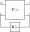
\includegraphics[width=0.5\linewidth]{generalized_plant}
						\caption{Generalized Plant Represenation}
						\label{fig:generalized_plant_representation}
					\end{figure}
				\end{column}
			\end{columns}
			$w$ are the inputs, $z$ are the error signals to be minimized, $u$ are the manipulated variables, $v$ are the measurement signals, $\mathbf{P}(s)$ is the open loop plant, and $\mathbf{K}(s)$ is the closed-loop regulator.
%			\begin{columns}[onlytextwidth]
%				\begin{column}{0.5\textwidth}
%					
%				\end{column}
%				\begin{column}{0.5\textwidth}
%					
%				\end{column}
%			\end{columns}
			The close-loop response can be written as
			\begin{equation}
				z=\mathbf{G}(s)w\,,
			\end{equation}
			%			where $\mathbf{G}(s) = P_{11}(s) + P_{12}(s)\mathbf{K}(s)\left(I-P_{22}(s)\mathbf{K}(s)\right)^{-1}P_{21}(s)$ is the closed-loop transfer function matrix of the system.
			where $\mathbf{G}(s)$ is the transfer function matrix from the inputs $w$ to the errors $z$.
			$\mathcal{H}_\infty$ synthesis will then generate a regulator, which minimizes the $\mathcal{H}_\infty$ norm of the closed-loop transfer function $\mathbf{G}(s)$.
			For readers who are interested in the interpretation of the $\mathcal{H}_\infty$ norm, please refer to external resources such as Refs.~\cite{Thomas:2019, multivariable_feedback_control}.
			\end{block}
		\end{column}
		
		% Column 2
		\begin{column}{0.32\linewidth}
			\begin{block}{Methodology: Complementary Filter Problem as an $\mathcal{H}_\infty$ Problem (cont.)}
			
		
		
%			The $\mathcal{H}_\infty$ norm of the transfer function matrix is defined by
%			\begin{equation}
%				\left\Vert\mathbf{G}(j\omega)\right\Vert_\infty = \sup_\omega\left(\bar\sigma(\mathbf{G}(j\omega))\right)\,,
%			\end{equation}
%			where $j$ denotes the imaginary number, $\omega$ is the angular frequency, $\sup$ denotes the supremum, and $\bar\sigma(\mathbf{G}(j\omega))$ is the maximum singular value of $\mathbf{G}(s)$ at $\omega$.
			
			\medskip
			
			\begin{columns}[t, onlytextwidth]
				\begin{column}{0.45\textwidth}
%					Although everything about $\mathcal{H}_\infty$ method so far has been discussed under the context of feedback control, it can also be used to synthesize complementary filters.
					Consider the generalized plant architecture as shown in Fig.~\ref{fig:generlized_plant_complementary_filter}, which has a slight modification compared to that of Ref.~\cite{Thomas:2019}.
					Here, $\Phi_1$ and $\Phi_2$ are some uncorrelated stochastic processes with unit variance.
					$\hat{N}_1(s)$ and $\hat{N}_2(s)$ are transfer function models of the ASD of the noises $N_1$ and $N_2$.
					$W_1(s)$ and $W_2(s)$ are some weighting functions, which can be used to specify the (inverse) frequency-dependent specification of the sensing noises $N_1$ and $N_2$ respectively.
				\end{column}
				\begin{column}{0.5\textwidth}
					\begin{figure}[!h]
						\centering
						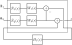
\includegraphics[width=1\linewidth]{generalized_plant_complementary_filter}
						\caption{Generalized plant representation for complementary filter synthesis.}
						\label{fig:generlized_plant_complementary_filter}
					\end{figure}
				\end{column}
			\end{columns}
		
			\medskip
			
			Minimizing the $\mathcal{H}_\infty$ norm of this plant will give optimal filters $H_1(s)$ and $H_2(s)\equiv 1-H_1(s)$ that best filter the noises $N_1$ and $N_2$ according to the specifications.
			It follows that, by setting $W_1(s)=1/\hat{N}_2(s)$ and $W_2(s)=1/\hat{N}_1(s)$, the requirements of $N_1$ is set to $N_2$ when $N_1\gg N_2$, and vice versa.
			These weights are reasonable specifications if there's no specific requirements for the sensing noises because over-suppressing one of the noises is not useful, i.e. there exists a lower bound defined by the either $N_1$ or $N_2$, whichever is lower.
			
%			The closed-loop transfer function reads
%			\begin{equation}
%				\mathbf{G}(s) = \begin{bmatrix}H_1(s)\hat{N}_1(s)W_1(s) & H_2(s)\hat{N}_2(s)W_2(s)\end{bmatrix}\,,
%			\end{equation}
%			where we've substitute $(1-H_1(s))$ with $H_2(s)$ due to Eqn.~\eqref{eqn:complementary}.
%			
%			\medskip
%			
%			The plant has a maximum singular value of
%			\begin{equation}
%				\bar\sigma(\mathbf{G}(j\omega)) \approx \max{(H_1(j\omega)\hat{N}_1(j\omega)W_1(j\omega),H_2(j\omega)\hat{N}_2(j\omega)W_2(j\omega))}\,,
%			\end{equation}
%			Now, if we set $W_1(s)=1/\hat{N}_2(s)$ and $W_2(s)=1/\hat{N}_1(s)$, then $\bar\sigma(\mathbf{G}(s))$ can be interpreted as the ratio between the super sensor noise and the lower bound of the sensing noise, assuming that the super sensor noise is dominated one of the filtered sensing noises, which is generally true except at the cross-over frequency.
%			Minimizing the $\mathcal{H}_\infty$ norm would then be approximately minimizing the maximum difference of the log super sensor noise and the log noise lower bound.
			\end{block}
			
			\begin{block}{Results: Synthesizing Complementary Filters for SRM in KAGRA}
				\begin{columns}[t, onlytextwidth]
					\begin{column}{0.55\textwidth}
						The proposed method is exemplified with sensing noises taken from the preisolator of the signal-recycling mirror (SRM) in KAGRA.
						The complementary filters previously designed in Refs.~\cite{Sekiguchi:2016bmv,vanHeijningen:2018cpc} are also compared with that synthesized by the proposed method.
						
						The amplitude spectral densities (ASDs) of the sensing noises $N_1$ and $N_2$ and the transfer function models $\hat{N}_1(s)$ and $\hat{N}_2(s)$ are shown in Fig.~\ref{fig:noise_fit}.
						Here, $N_1$ denotes quadrature sum of the relative displacement sensor (LVDT) self-noise and the mean seismic noise at KAGRA taken from Ref.~\cite{seismic_noise_of_kagra}, whereas $N_2$ is the geophone self-noise.
					\end{column}
					\begin{column}{0.45\textwidth}
						\begin{figure}
							\centering
							\includegraphics[width=1\linewidth]{noise_fit}
							\caption{Sensing noises of the SRM preisolator sensors.}
%							\caption{Sensing noises of the SRM preisolator sensors. Blue solid: seismic noise coupled LVDT readout noise ($N_1$). Yellow dashed: transfer function model of $N_1$. Green solid: geophone self-noise $N_2$. Purple dahsed: transfer function model of $N_2$.}
							\label{fig:noise_fit}
						\end{figure}
					\end{column}
				\end{columns}
				
				\begin{columns}[onlytextwidth]
					\begin{column}{0.5\textwidth}
						\begin{figure}
							\centering
							\includegraphics[width=1\linewidth]{complementary_filters_hinfinity}
							\caption{Filters synthesized using $\mathcal{H}_\infty$ method.}
							\label{fig:complementary_filters_hinfinity}
						\end{figure}
					\end{column}
					\begin{column}{0.5\textwidth}
						\begin{figure}
							\centering
							\includegraphics[width=1\linewidth]{super_sensor_noise_tf}
							\caption{Predicted super sensor noise}
							\label{fig:super_sensor_noise_tf}
						\end{figure}
					\end{column}
				\end{columns}
				
				\medskip
				
				With the noise models $\hat{N}_1(s)$ and $\hat{N}_2(s)$, complementary filters are synthesized using $\mathcal{H}_\infty$ method with no information other than the sensing noises themselves.
				The resulting complementary filters are shown in Fig.~\ref{fig:complementary_filters_hinfinity}.
				
				\medskip
				
				Fig.~\ref{fig:super_sensor_noise_tf} shows the predicted ASD of the super sensor noise (in green) defined by
				\begin{equation}
					\left\vert \hat{N}_\text{super}(j\omega)\right\vert = \left[\left\vert H_1(j\omega)\right\vert^2\left\vert \hat{N}_1(j\omega)\right\vert^2 + \left\vert H_2(j\omega)\right\vert^2\left\vert \hat{N}_2(j\omega)\right\vert^2\right]^{\frac{1}{2}}\,.
				\end{equation}
				The super sensor noise here follows the shape of the lower bound of the sensing noises at all frequencies, which would indicate that the order of roll-off is critical at all frequencies.
			\end{block}
		\end{column}
	
		% Column 3
		\begin{column}{0.32\linewidth}
			\begin{block}{Results: Synthesizing Complementary Filters for SRM in KAGRA (Cont.)}
				
				%				As can be seen, notch-like feature at around $0.2\,\text{Hz}$ is present in the low pass filter.
				%				complementary filters from advanced LIGO \cite{Matichard:2015} and Virgo \cite{low_frequency_optimization_and_performance_of_advanced_virgo_seismic_isolation_system} also exhibit similar behavior, but the feature is clearly missing from that of \cite{Sekiguchi:2016bmv} and \cite{vanHeijningen:2018cpc}.
				%				This is a designed feature to provide additional seismic noise attenuation in the relative displacement sensor readout.
				%				Using the proposed method, we arrived at the same design feature by optimization using no additional information rather than the sensing noise themselves.
			In Fig.~\ref{fig:super_sensor_noise_comparison}, we compare noise performance of the complementary filters from Ref.~\cite{Sekiguchi:2016bmv}, Ref.~\cite{vanHeijningen:2018cpc}, and the proposed method, and the super sensor nosies are denoted $N_\text{super, 1}$, $N_\text{super, 2}$, and $N_{\text{super},\mathcal{H}_\infty}$ respectively.
			The super sensor noises are calculated directly use the quadrature sum of the filtered noises $\vert H_1(j\omega)\vert N_1$ and $\vert H_2(j\omega)\vert N_2$.
			
			\medskip
			
			\begin{columns}[onlytextwidth]
				\begin{column}{0.45\textwidth}
					The cross-over frequency of the filters in Refs.~\cite{Sekiguchi:2016bmv, vanHeijningen:2018cpc} are set to be the cross-over frequency of the sensing noises in Fig.~\ref{fig:noise_fit}, which is 0.0898 Hz in this case, as recommended in Ref.~\cite{Sekiguchi:2016bmv}.
					The ASD of the super sensor noise from $\mathcal{H}_\infty$ filters is on par, if not lower, compared to the other two below $0.4\,\text{Hz}$ but is slightly higher at higher frequencies.
					The shape of $N_{\text{super}, \mathcal{H}_\infty}$ at higher frequencies still follows that of the lower bound, which again, indicating that the sensing noises are critically rolled off.
				\end{column}
				\begin{column}{0.5\textwidth}
					\begin{figure}
						\centering
						\includegraphics[width=1\linewidth]{super_sensor_noise_comparison}
						\caption{Comparison between the super sensor noises predicted using filter design from \cite{Sekiguchi:2016bmv, vanHeijningen:2018cpc} and the proposed method.}
						\label{fig:super_sensor_noise_comparison}
					\end{figure}
				\end{column}
			\end{columns}

			\medskip
			
			Performance indices are compared in Table.~\ref{table:metrics}, including the super sensor noises' RMS (overall noise performance), the band-limited RMS around 0.1 to 0.5 Hz (seismic noise attenuation performance at microseism), and the ASD at 10 Hz (potential feedback control limit).
			\begin{table}
				\begin{tabular}{|c|c|c|c|}
					\hline
					& RMS ($\mu\text{m}$) & RMS (0.1-0.5 Hz) ($\mu\text{m}$)& ASD (10 Hz) ($\mu\text{m}/\sqrt{\text{Hz}}$)\\
					\hline
					$N_\text{super, 1}$ & 0.5895 & 0.2400 & 4.443e-6\\
					\hline
					$N_\text{super, 2}$ & 0.4726 & 0.1650 & 4.443e-6\\
					\hline
					$N_{\text{super}, \mathcal{H}_\infty}$ & 0.3631 & 0.1041 & 2.087e-5\\
					\hline
					Lower bound & 0.0462 & 0.01422 & 4.443e-6\\
					\hline
				\end{tabular}
				\caption{RMS, band-limited RMS, and ASD values at 10 Hz of the super sensor noises predicted using filter design from \cite{Sekiguchi:2016bmv,vanHeijningen:2018cpc} and the proposed method (\textbf{lower the better}).}
				\label{table:metrics}
			\end{table}
			The $\mathcal{H}_\infty$ complementary filters perform better than the other two complementary filters in terms of RMS value especially at the microseism band, which makes it a better candidate for active seismic noise isolation.
			While it performs worse at 10 Hz, there's still a 3 orders of magnitude reduction compared to that of the LVDT self-noise ($\approx\, 10^{-2}\,\mu\text{m}/\sqrt{\text{Hz}}$).
			\end{block}
			\begin{block}{Conclusion}
				\begin{itemize}
					\item The complementary filter problem is formulated as an $\mathcal{H}_\infty$ optimization problem.
					\item Complementary filters can be synthesized using $\mathcal{H}_\infty$ method with no information other than the sensing noises themselves.
					\item The method is exemplified using SRM preisolator sensors and is shown to able to generate filters that better reduce the RMS of the super sensor noise especially around the microseism band.
					\item While the $\mathcal{H}_\infty$ filters perform worse at 10 Hz, 3 orders of magnitude reduction in super sensor noise ASD (compared to LVDT) can still be achieved.
				\end{itemize}
			\end{block}
			\begin{block}{References}
				\bibliographystyle{unsrt}
				\bibliography{poster_terrence_tak_lun_tsang}
			\end{block}
		\end{column}
	\end{columns}
\end{frame}
\end{document}
